\chapter{System design}
\label{chap:System design}
%Hvad dette chapter skal indeholde:
%Hvordan positionen på robotten bliver udregnet og evt hvordan den skal kunne bevæge sig?????(referer og citer hvad vi har skrevet i incerement two)
%Hvordan vi skal have Kinect og Arduino til at snakke sammen(Program i kinect der sender data til wifishield som arduinoet kan bruge)
%Skal vi have noget med afgrænsningen til at vi bouncer med her????
%Hvordan vores schedule skal fungere? Teorien bag det også kan det blive forklaret i implementationen.
%I system design skal vi også snakke om memory management evt ?? 
%Skal vi skirve om den billede analyse som kinecten laver??
This chapter will describe some of the software choices made, as well as the robot design. The program design, the robots positioning and movement and how the Arduino and Kinect are connected, will also be described in this chapter. 

\section{Software choices}
\label{sec:Software choices}
%Hviket software vi bruger til at udvikle robotten og hvilke libraries vi bruger? SKal vi evt. have en section om Hardware choices? Skal vi skrive her at vi bruger Arduino's ide og at vi bruger 1.0.3??

In this section the software choices made for the Arduino IDE will be described. Also, the libraries used for making the program will be described as well. 

\subsection{Arduino IDE}
\label{sec:Arduino IDE}
After testing the Arduino IDE 1.6.12 with the code defined on the Arduino website's Wifi-guide \citep{wg}, it was discovered that the Wifi library was not compatible in the IDE in a series of newer versions. The library was supported in version 1.0.3, which is why this particular IDE version is used in this project. The newer IDE's has increased security, which would actively refuse any TCP connection from the computer.

\subsection{Libraries}
\label{sec:Libraries}
To be able to use the Motor- and Wifi shield, two libraries had to be included to the project. This gave some new functions, be to able to make the program. 

\subsubsection{Motor.h}
\label{sec:Motor.h}
The Motor.h library is being used for the project, making it possible to control the motors independently of each other, e.g. the motors can have set different speeds and can be stopped at different times. If the library was not included in this project, the group had to write their own code to control the motors and reading the motor encoders. 

\subsubsection{Wifi.h}
\label{sec:Wifi.h}
Arduino Wifi library is used to create the connection between the Wifi shield and the router. This library has methods for creating a server, where clients can both read from and write to the server. The subsection \ref{sec:Arduino IDE} explains complications between the versions of the Arduino IDE, and why the Arduino IDE 1.0.3 is used for this project.

\section{Robot design}
\label{sec:Robot design}
%Kort om hvordan vi har lavet robotten? Vi kan evt. have noget med hvordan vi placere vores kinect i en subsection?
The purpose of the robot is to catch the thrown object, by driving to the impact point of the object and the ground within the predefined area. The final design of the robot is shown in figure \ref{robot}.

\begin{figure}[h]
	\centering
	\fbox{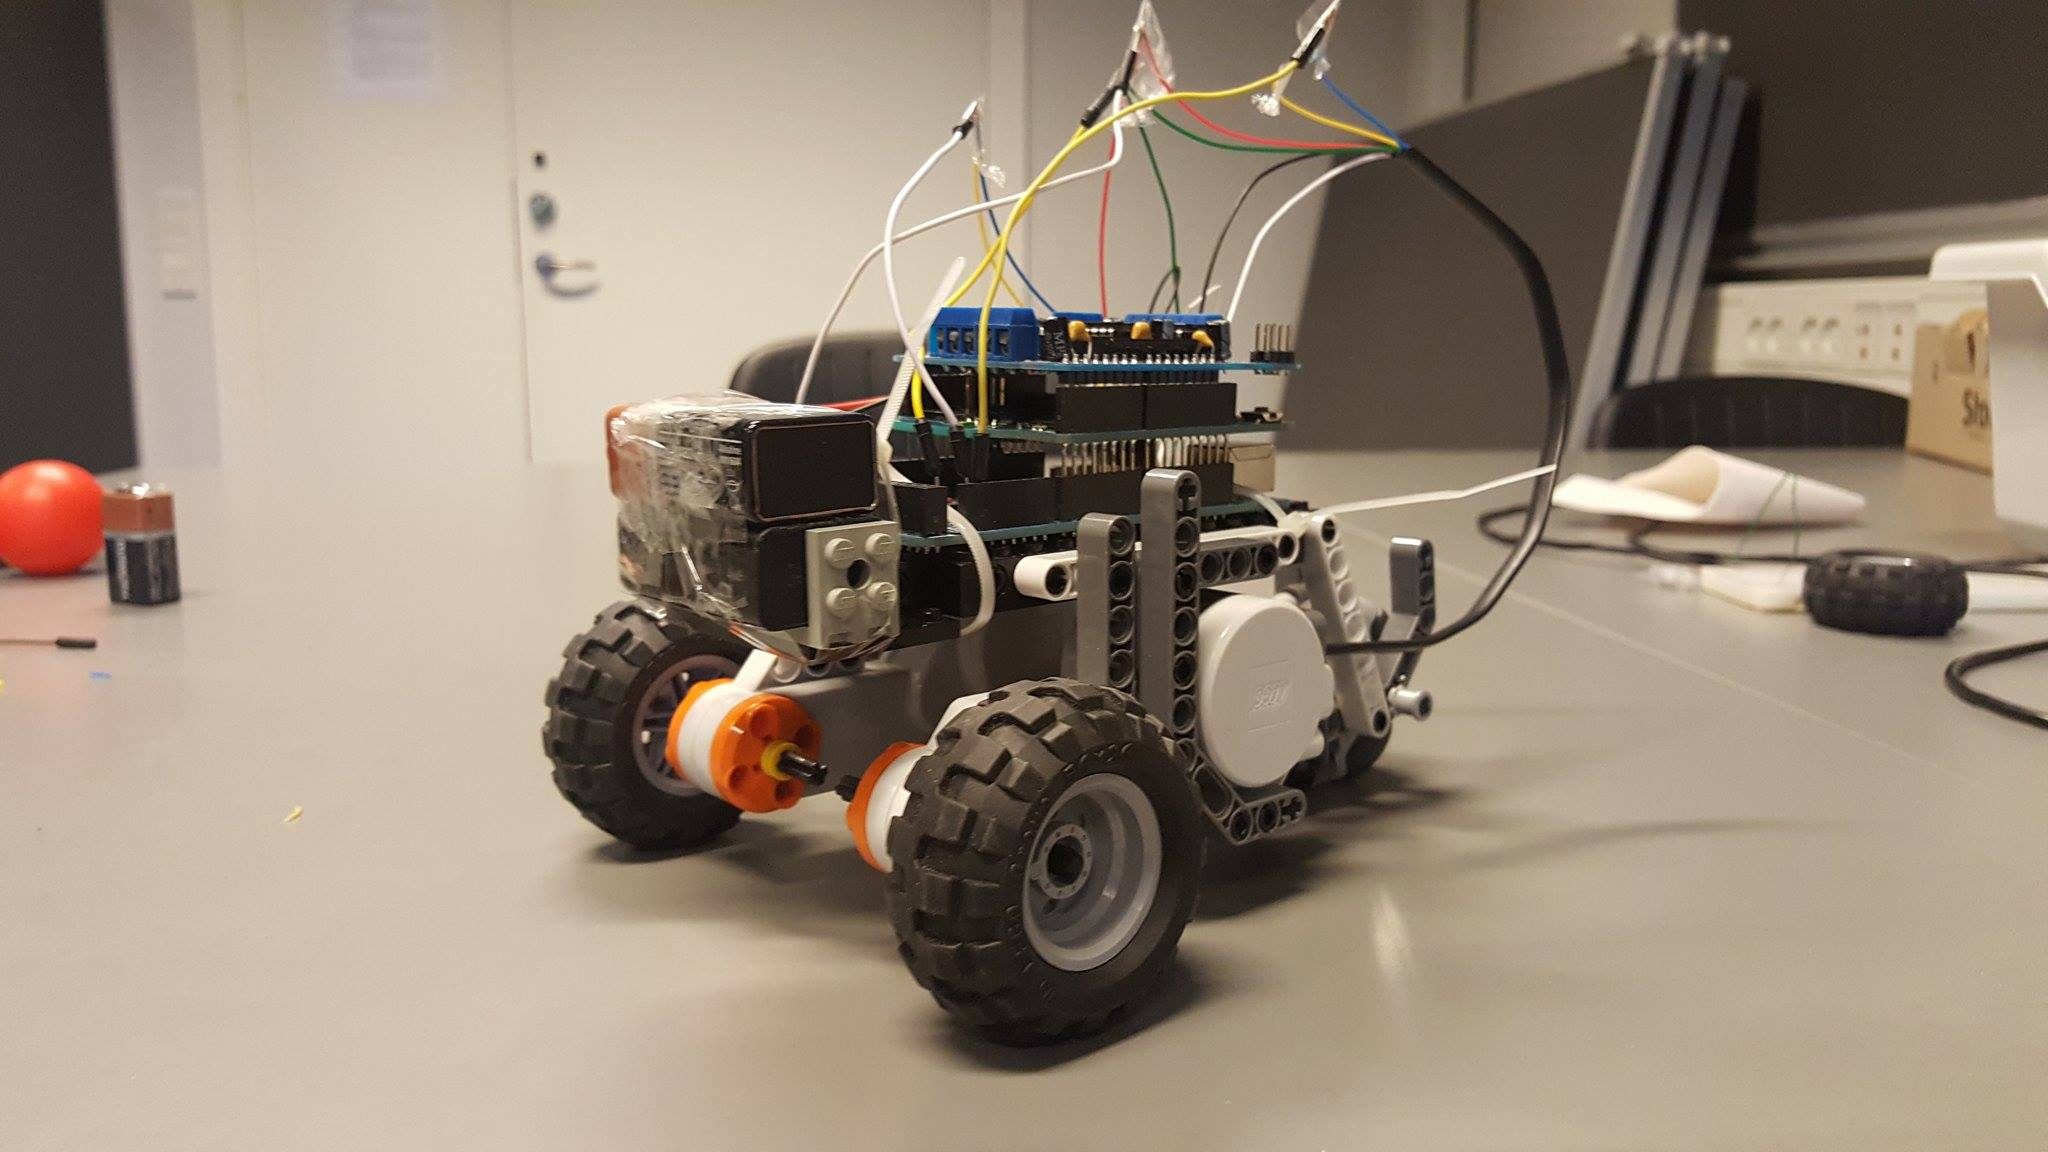
\includegraphics[scale=0.20]{billeder/robot}}
	\caption{The final design of the robot}
	\label{robot}
\end{figure}

The robot uses two LEGO NXT Servo motors with corresponding wheels, which will act as the front wheels. The back wheel can slide from side to side, which is important, since the wheel will be dragged sideways when the robots turns, whereas a normal rubber wheel would have caused a lot of friction. 
The robot is build around the NXT Servo motors, having a kind of platform at the top. The Arduino is stripped to the platform, with the shields on top of it. This ensures that the Arduino does not slide off the robot while moving.
The robot was build with the arduino at the top, for easy access to the different pins if needed. 

\section{Arduino program design}
\label{sec:Arduino program design}
%Dette kan indeholde hvad vores program skal kunne gøre og evt. en punktform over hvilke funktioner/tasks som programmet løber i gennem.
As mentioned in section \ref{sec:Software choices}, the arduino program was developed in the Arduino IDE version 1.0.3. The program will be responsible to communicate to the robot where to move, to reach the collision point, sent by the Kinect of the object thrown at its predefined area. This is done by the program translating the coordinates from the Kinect, into coordinates know for the robot and move to that specific location

The program have a setup and will loop the behavior of the robot. First the setup function, sets up the WiFi connection to the Kinect program, it then waits for the Kinect program to send coordinates for the impact point of the object thrown. When it has received a set of coordinates, it will then translate the coordinates to so it knows where to move to. The next steps, the arduino program will continuously loop through until the program are exited: First it will check if it is at the impact point, if it is, the program is done. Else the robot will start moving, while it keeps adjusting it direction relative to the robots heading. Finally in the loop it will update the robots current position and its heading. All this can be broken down into tasks:

\begin{itemize}
	\item Make connection to the Kinect
	\item Wait to receive coordinates from the Kinect
	\item When the coordinates are received, it will translate these to understandable coordinates for the arduino and then enter the behavioral loop function:
	\begin{itemize}
		\item Check if already at the collision point, if it is exit program
		\item Start moving, adjust direction relative to heading
		\item Update the its position
	\end{itemize}
\end{itemize}
 
\begin{figure}[h]
	\centering
	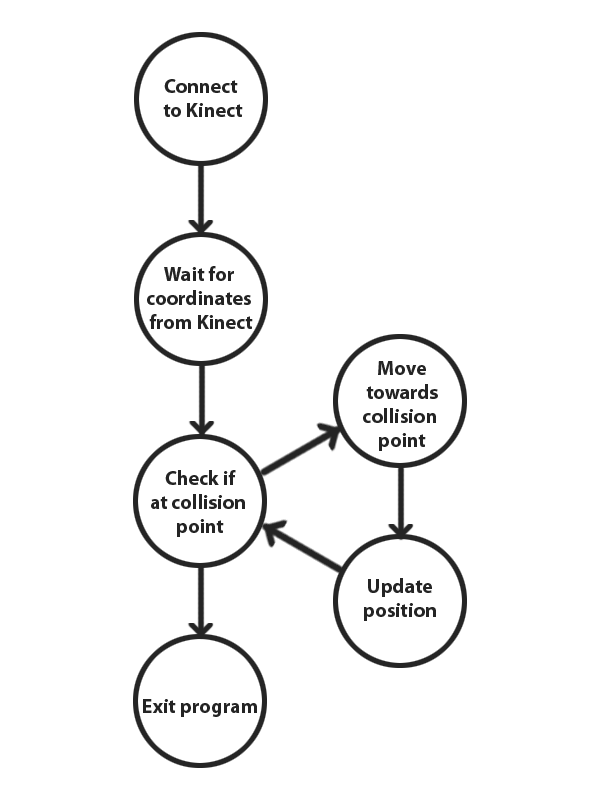
\includegraphics[scale=0.25]{billeder/flowgraph.png}
	\caption{The flowgraph of the program}
	\label{figure:flowgraph}
\end{figure}

\section{Robot positioning and movement}
\label{sec:Robot positioning and movement}
%Kan indeholde hvordan vi har tænkt os med robottens kordinatsystem og hvordan den skal bevæge sig op i mod det punkt som den får fra kinecten.
The idea for moving the robot would be to send coordinates to the robot, which would be converted to explicit millimetre values of the distance from the starting point (0, 0). This starting point delimits a predefined area, as described in Appendix \ref{sec:i1Predefined areaImplementation}, which is the area in which the robot should catch the thrown object. This area is defined by the robots capabilities and limitation. This area would allow the robot to calculate the distance travelled, and compare that value to the distance of the received coordinate. The NXT Servo motor encoders should be used to calculate the distance travelled. \newline
If the robot has read a coordinate and started to move towards it, receiving a new coordinate would redirect the robot to the new coordinate instead. As described in Appendix \ref{sec:i1MovementImplementation}, the robots maximum speed was 25.5 cm/s, but it was significantly slower moving backwards than forwards. This resulted in the definition of the robot always starting at the coordinate (0, 0), and not considering any trash thrown behind the robot. The predefined area was determined to only be in front of the robot, to ensure that the robot does not move backwards. 

\section{Connecting Arduino and Kinect}
\label{sec:Connecting Arduino and Kinect}
%Kan indeholde hvordan vi har tænkt os at de skal kunne snakke sammen og hvilket data der skal blive sendt i mellem dem.
For convenience, and as a part of the requirements for this project, the Arduino should receive wireless data from a computer, connected to the Kinect. The Arduino Wifi Shield makes this possible, with the Wifi library included in the Arduino IDE. \newline
The connection between the Arduino and the computer should be through a local router, with a set SSID and password. The computer should use the Kinect to calculate an impact point of the object, and send this in a specific format, so that the data can be easily read and translated to a set of coordinates for the robots movement. The computer should be able to send coordinates more than once, since the first impact point is not necessarily be precise enough to catch the object. The computer should calculate increasingly accurate impact points, which should be sent with a certain minimal inter-arrival time, to not hinder the robots movement, and yet still in time for the robot to correct itself. \newline
The Arduino should receive this data and read whenever it has sufficient time to do so, and convert the data received to match the right coordinate in the predefined area. 

\section{Scheduling}
\label{sec:Scheduling}
%Snakke om de forskellige tasks, deres deadlines og hvliken metode vi vil bruge til at schedule?
The subsections Cyclic Executive, Interrupts and their definitions, Stack Overflow, Interrupt Overload and Real-Time analysis all uses the the article "Safe and Structured Use of Interrupts in Real-Time and
Embedded Software" written by John Regehr. \citep{safe}


\subsection{Cyclic Executive}
\label{sec:Cyclic Executive}
A cyclic executive is a model which assumes a fixed set of periodic tasks. The model is about designing an entirely static schedule in which the tasks are cyclically executed at their rate, since they are periodic, and must also meet their deadline. The model is cyclic since when the last task ends and the allotted time of a cycle ends, a new cycle begins, with all tasks placed in the same specific order as the previous cycle. The creation of such a schedule proves by construction that the tasks will always meet their deadlines at runtime, if the assumptions of the model are true. \newline
To ensure that the cyclic executive is in synchronization with real elapsed time, synchronization points are inserted into the code that implements it (maybe give an example of us doing so, or at least mention it)
Once cyclic executives are constructed, the implementation is simple and efficient since there is little overhead since there is no scheduling at runtime. Cyclic executives can be constructed separately from the system, by hand or by a tool.

\subsection{Interrupts and their definition}
\label{sec:Interrupts and their definition}
To talk about interrupts we first need to define what we are talking about, these definitions are quotes from the John Regehr's article \citep{safe}. The definition for an interrupt is twofold, as the first part is as follows:

{\addtolength{\leftskip}{10 mm}
	\enquote{A hardware-supported asynchronous transfer of control to an interrupt vector based on the signaling of some condition external to the processor core}\\*
	
}

The second part of the definition is:

{\addtolength{\leftskip}{10 mm}
	\enquote{An interrupt is the execution of an interrupt handler: code that is reachable from an interrupt vector}\\*
	
}

The definition for the introduced term interrupt vector:

{\addtolength{\leftskip}{10 mm}
	\enquote{A dedicated or configurable location in memory that specifies the address to which execution should jump when an interrupt occurs}\\*
	
}

Interrupts often but not always return control flow to where, the interrupt disrupted control flow. Interrupts often change the state of main memory, and that of device drivers, but does not disturb the main processor context of the computation which was disturbed.\newline
A interrupt is pending when it's firing condition has occurred, the interrupt controller has been updated and the interrupt handler has not started executing. A missed interrupt is when the firing condition occurs but it does not become pending, this is usually because the interrupt is currently pending. Most hardware platforms. including the atmega2560, use a bit to distinguish whether an interrupt is pending or not. Hardware support can be used to disable interrupts by manipulating bits in hardware registers either through the master interrupt enable bit, or the enable bits for each interrupt. 

The following conditions decide when the firing condition for an interrupt is true:

\begin{itemize}
	\item The interrupt is pending
	\item The processors master interrupt enable bit is set
	\item The enable bit for each interrupt bit is set
	\item The processor is in between executing instructions
	\item There exists no higher priority interrupt which fulfills 1-4.
\end{itemize}

Another important part of interrupts is interrupt latency, which is the time between the interrupt firing conditions become true, and the first instruction of the interrupt handler has begun executing. Nested interrupts is when an interrupt handler is preempted by another interrupt. An important distinction between threads and interrupts is that thread scheduling is through software, while interrupt scheduling is through hardware interrupt controller.

\subsection{Stack Overflow}
\label{sec:Stack Overflow}
A stack overflow is when a stack grows beyond the confines of the memory allocated to it, thereby corrupting RAM and could cause system malfunction and crash. Allocating memory to a stack is about a balance between enough memory to prevent stack overflow from occurring and not assigning more memory than needed. There are two ways to approach this problem, analysis- and testing based. A significant advantage of analysis is that it can be performed quickly through tools, in contrast to testing which is much more laborious. \newline
The testing approach is about running the system and observing how large the stack grows. This approach is a kind of black box testing, it doesn’t matter how or why memory is used, all that matters is how big the stacks becomes. A problem with the testing based approach is that it can miss some of the program paths, where it might have taken a shorter branch at some point during the execution of the program. \newline
The analysis based approach is concerned with the control flow and its goal is to find the path which pushes the most data onto the stack. The problem with the analysis based approach is that it's often too optimistic about the maximum stack size to prevent stack overflow. \newline
Stack overflow is a general problem in embedded systems, but will not be a problem for this project. A common factor that leads to this, is that threads will have allocated memory and in a system with many interrupts, the interrupts can cause the memory which was allocated to the thread to overflow. The arduino mega2560 board used in this project is not using multiple threads, have relatively large memory and does not use more than one type of interrupt which cannot preempt itself. 

\subsection{Interrupt overload}
\label{sec:Interrupt overload}


Interrupt overload is when interrupts occur so frequently they dominate the processor from performing its other computations, which in the worst case can end up starving other important processes. While it may be intuitive to think that large interrupt payloads are a natural cause of interrupt overload, but it is rather unexpectedly large interrupt loads which can cause interrupt overload. A reliable maximum interrupt request rate is a important thing to ensure that it is accurately evaluated to have a reliable real-time system.


To discover if the interrupt overload can occur, it is possible to analyze how much cpu utilization can be spent handling interrupts. If the cpu utilization for handling interrupts is above 100% then the cpu might not be able to handle all interrupts, neglecting the rest of the system entirely. If the cpu utilization is below 100%, the rest of the system also needs cpu utilization which means the net utilization could become greater than 100% resulting in interrupt overloading starving other functions.
To prevent an interrupt overload from starving other functions,
The maximum time spent in an interrupt handler can be calculated by the maximum execution time of a given interrupt multiplied by the worst-case arrival rate. 

The maximum execution time of the in interrupt handler in our system is 40 clock cycles and the worst-case arrival rate is 1 occurrence per millisecond. The worst-case arrival rate is based on the maximum speed of the NXT servo motor and the motor encoder which reads it, which causes interrupts to be generated. \newline
The maximum time spent in an interrupt handler in our system is \begin{math} \frac{40 \cdot 1}{16000} = 0.0025\% \end{math} of cpu spent dealing with interrupts, where the 16.000 comes from the cpu clock cycles per millisecond. The interrupts in this project listens to the motor encoders for change, each time a change happens(the change is between high and low voltage), it will interrupt the program and in this project it will increment a counter. Since only one type of interrupt with relatively low amount of cpu utilization is used, this type of problem doesn’t occur. 

Real-Time analysis 

The previously addressed problems of stack overflow and interrupt overload are subproblems of the real-time schedulability analysis, especially concerning interrupts, which will make sure that all computations will be met within their time constraints. 
To schedule the system a cyclic executive is used, which is mentioned in section \ref{sec:Cyclic Executive}, which handles many of the problems addressed, as long as its assumptions are true. 
Since the cyclic executive has predetermined behaviour it will have low jitter for the execution of each of the periodic tasks. Although jitter has not been a particular concern in this project.\newline Jitter is the concept of time variation in a computed output being messaged to external environment from period to period.
The strengths of using a cyclic executive include: execution schedule is predetermined, simple, efficient and fast, low jitter, prevents race-conditions and deadlock(not sure if true, seems true). 
The very existence of a cyclic executive is a proof by construction that the real-time analysis will hold, and the problems which arise from interrupts have also been addressed in this chapter.